\documentclass[conference,10pt]{IEEEtran}
\IEEEoverridecommandlockouts
\usepackage[utf8]{inputenc}
\usepackage{newtxtext,newtxmath}
\usepackage[dvipsnames,svgnames,x11names,hyperref]{xcolor}
\usepackage[T1]{fontenc}
\usepackage{array}
\usepackage{url}
\usepackage{graphicx}
\usepackage{algorithmic}
\usepackage{hyperref}
\usepackage{microtype}
\usepackage{minted}
\usepackage[export]{adjustbox}
\usepackage{endnotes}
\usepackage{siunitx}
\usepackage{paralist}
\usepackage[linesnumbered,ruled,vlined,lined,boxed]{algorithm2e}
\usepackage[acronym,nohypertypes=acronym]{glossaries}

\ifCLASSOPTIONcompsoc
  \usepackage[caption=false, font=normalsize, labelfont=sf, textfont=sf]{subfig}
  \usepackage[nocompress]{cite}
\else
  \usepackage[caption=false, font=footnotesize]{subfig}
  \usepackage{cite}
\fi

\usepackage[capitalise]{cleveref}

\setacronymstyle{long-short}

\def\UrlBreaks{\do\/\do-\do.\do_}
\def\UrlNoBreaks{\do:}

%\let\footnote=\endnote

\newcommand{\papertitle}{SenSQL: Networked Storage and Query Processing for Spatiotemporal Sensor Data}

\newacronym{iot}{IoT}{Internet of Things}
\newacronym{sql}{SQL}{Structured Query Language}
\newacronym{lost}{LoST}{Location-to-Service Translation}
\newacronym{gd}{GD}{Geographic Discovery Service}
\newacronym{acps}{ACPS}{autonomous cyber-physical system}
\newacronym{dbms}{DBMS}{database management system}
\newacronym{senml}{SenML}{Sensor Markup Language}
\newacronym{lan}{LAN}{local area network}
\newacronym{wan}{WAN}{wide area network}
\newacronym{wgs}{WGS}{World Geodetic System}
\newacronym{gps}{GPS}{Global Positioning System}
\newacronym{uri}{URI}{Uniform Resource Identifier}
\newacronym{ip}{IP}{Internet Protocol}
\newacronym{dns}{DNS}{Domain Name System}
\newacronym{de9im}{DE-9IM}{Dimensionally Extended 9-Intersection Model}
\newacronym{cctld}{ccTLD}{country codey top-level domain}
\newacronym{ddds}{DDDS}{Dynamic Delegation Discovery System}
\newacronym{naptr}{NAPTR}{Naming Authority Pointer}
\newacronym{json}{JSON}{JavaScript Object Notation}
\newacronym{pm2.5}{PM2.5}{particulate matter}
\newacronym{srv}{SRV}{service record}

% Potential venues for publication:
%
% IFIP Networking 2021 (~ 23\%)
%  * Deadlines:
%    - Abstract: January 5, 2021 (https://edas.info/N27861)
%    - Paper: January 12, 2012
%  * Guidelines:
%    - 9 pages maximum
%    - double-blind review
%
% IEEE DCOSS 2021 (~ 25-30\%)
%  * Deadlines:
%    - Abstract: January 18, 2021 ( https://edas.info/newPaper.php?c=27882)
%    - Paper: January 25, 2021
%  * Guidelines:
%    - 8 pages maximum (2 additional at $100/page for appendices, theorems, implementation)
%    - single-blind review
%
% Usenix ATC 21
%  * Deadlines:
%    - Paper: January 12, 2021
%  * Guidelines:
%    - 11/5 pages maximum (without references)
%    - double-blind review

% Random Ideas:
% - The autonomous sensor system might store its own (private) spatial objects.
%   It may provide a means to select related sensors, but not necessary the spatial
%   objects themselves for privacy reasons. For example, you might ask for sensors
%   in the living room (pick a better example), but may not be able to obtain what
%   living room means. This is probably more useful in shared office building than
%   in apartments

\hypersetup{
  colorlinks=true,% Color URLs with urlcolor
  linkcolor=black,% The color for internal (cross-reference) links
  urlcolor=Blue4,% The color for URLs (hyperlinks)
  citecolor=black,
  pdftitle={\papertitle}
}

\urlstyle{same}

\begin{document}
\title{\papertitle}

\author{
  \IEEEauthorblockN{
    \href{mailto:janakj@cs.columbia.edu}{\color{black}Jan Janak},
    \href{mailto:hgs@cs.columbia.edu}{\color{black}Henning Schulzrinne}
  }
  \IEEEauthorblockA{
    Department of Computer Science, Columbia University, New York, USA
  }
  Email: \{janakj,hgs\}@cs.columbia.edu
}

\maketitle

\begin{abstract}
TBD
\end{abstract}

\glsresetall

\section{Introduction}\label{sec:introduction}

A cornerstone of every \gls{iot} system is its data acquisition infrastructure in the form of sensors. Sensors perform measurements and generate data representing measured quantities. The data is then used by applications that monitor on control the system. Some applications require a history of sensor measurements to function, e.g., to calculate aggregates or estimate trends. With the growing size and complexity of \gls{iot} systems, the need for a distributed sensor database with a generic query interface arises. Ideally, the database would be application-agnostic with a declarative query interface allowing the programmer to focus on what sensor data to get, rather than how to get it.

We propose a distributed \gls{sql} based storage and query processor architecture for heterogeneous \gls{iot} systems. Our architecture provides the application programmer with a familiar declarative \gls{sql} query interface to spatiotemporal sensor data that is geographically partitioned and distributed.

This work is part of our broader research effort to develop fundamental programming abstractions for heterogeneous \gls{iot} systems.

% Background
%  - introduce classes of sensors
%  - introduce device roles (e.g., storage node)
%  - SELECT-FROM-WHERE-GROUP BY-HAVING-ORDER BY-LIMIT

% Motivation
% - Limit bandwidth, allow sensors generate measurements frequently, transfer only when necessary
% - Compute aggregates close to the source of the data
% - Make aggregation a generic operation that can operate on any data
% - Support intuitive declarative-style interface for application programmers
% - Data functionality partitioning (for reliability purposes)
%
% Data Model

% aggregates
%  - data reduction mechanism
%  - summarization (e.g., for privacy)
%
% SQL is loosely based on a relational algebra
%
% Architecture
% - stateless versus stateful sensors
% - storage node
% - independent sensor system (associated with an administrative entity, a.k.a. principal)
% - coverage region
% - independent sensor system directory/router
%

\section{Related Work}\label{sec:related-work}

% Declarative query languages: SQL/MM, GraphQL, GeoSPARQL

% TinyDB: Cite the main (long) TinyDB paper and perhaps some of the earlier related papers
TinyDB \cite{madden2005tinydb} is a distributed query processor for ad hoc sensor networks. Similar to our work, TinyDB provides a generic \gls{sql}[-like] query interface for sensor data to applications. Unlike our architecture, TinyDB does not support spatial predicates, is designed to operate in a uniform environment, and its \gls{sql} dialect provides domain-specific primitives for ad hoc sensor networks, e.g., to control measurement data acquisition on energy constrained devices. The obvious drawback of acquisitional query processing is that data is only collected on demand, making it impossible to execute future queries over a history of samples.

Cougar \cite{yao2002cougar} was a similar distributed database architecture based on in-network aggregation and computation.

Sun and Zhou \cite{sun2010querying} discuss \gls{sql} extensions for ad hoc sensor networks. The extensions include operators motivated by the dynamic nature of ad hoc sensor networks.

Bacon et al. \cite{bacon2017spanner} discuss the evolution of Google Spanner---a globally-distributed, replicated, consistent database---from a key-value store into a relational \gls{sql}[-based] database system. Similar to our work, this paper discusses breaking a \gls{sql} query into sub-queries that could be send to shards.

The \gls{lost} Protocol~\cite{rfc5222} and the associated architectural framework \cite{rfc5012,rfc5582} might serve as a good starting point for the design and implementation of the \gls{gd}.

\gls{senml}~\cite{rfc8428} might provide inspiration for a general spatiotemporal sensor measurement data model.

Tsiftes and Dunkles \cite{tsiftes11:sensordb} discuss the design of Antelope, a \gls{dbms} designed to run on a constrained device. Their approach complements TinyDB and Courage discussed above.

Bolt \cite{gupta14:bolt} is a time-series database for connected homes. Data sharing via untrusted storage servers is interesting and potentially somewhat relevant for our work.

Cockroach Labs discuss spatial indexing and sharding on their blog \cite{cockroach-spatial-indexing}. The article offers interesting insights on spatial partitioning that might be relevant for this work.

\nocite{pavlo2016s}

\begin{figure}
  \centering
  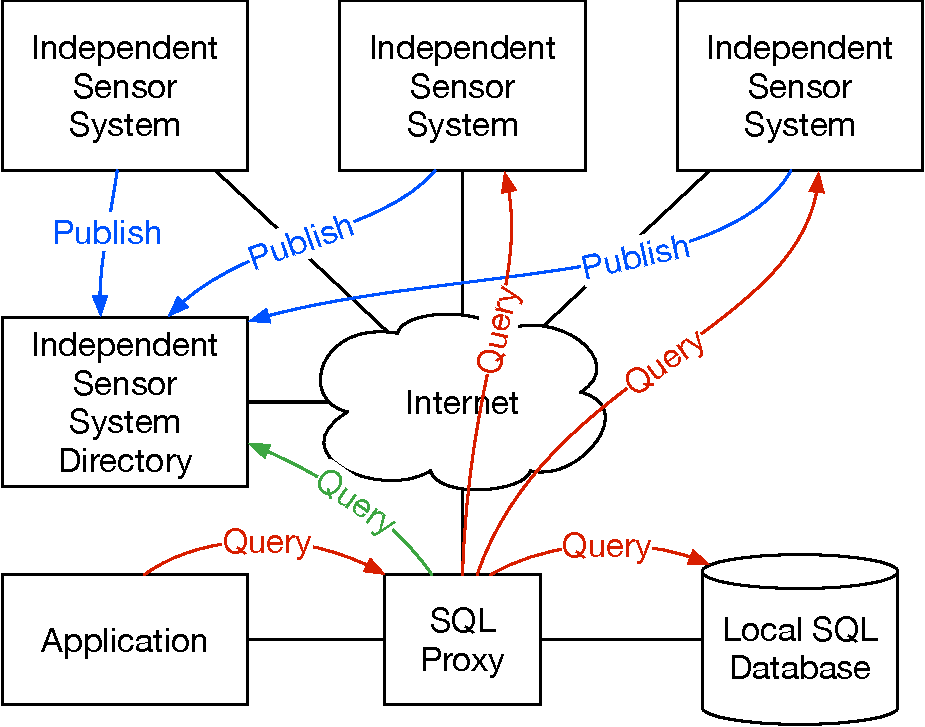
\includegraphics[width=0.7\linewidth]{figs/conceptual-diagram.pdf}%
  \caption{SenSQL as a federation of \glsfirstplural{acps} discoverable via the \glsfirst{gd}.}\label{fig:conceptual-diagram}
\end{figure}

\section{Autonomous Cyber-Physical System}\label{sec:autonomous-cyber-physical-system}
\begin{figure}
    \centering
    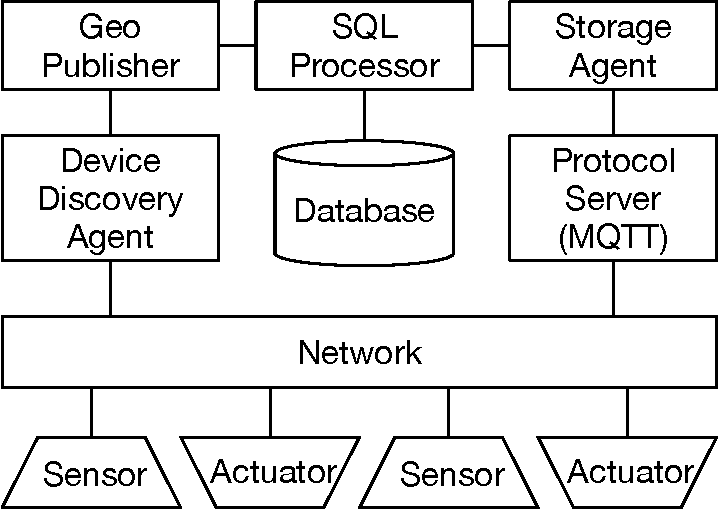
\includegraphics[width=0.8\linewidth]{figs/acps.pdf}%
    \caption{The conceptual diagram of an autonomous cyber-physical system (ACPS).}\label{fig:acps}%
\end{figure}

\begin{figure}
    \centering
    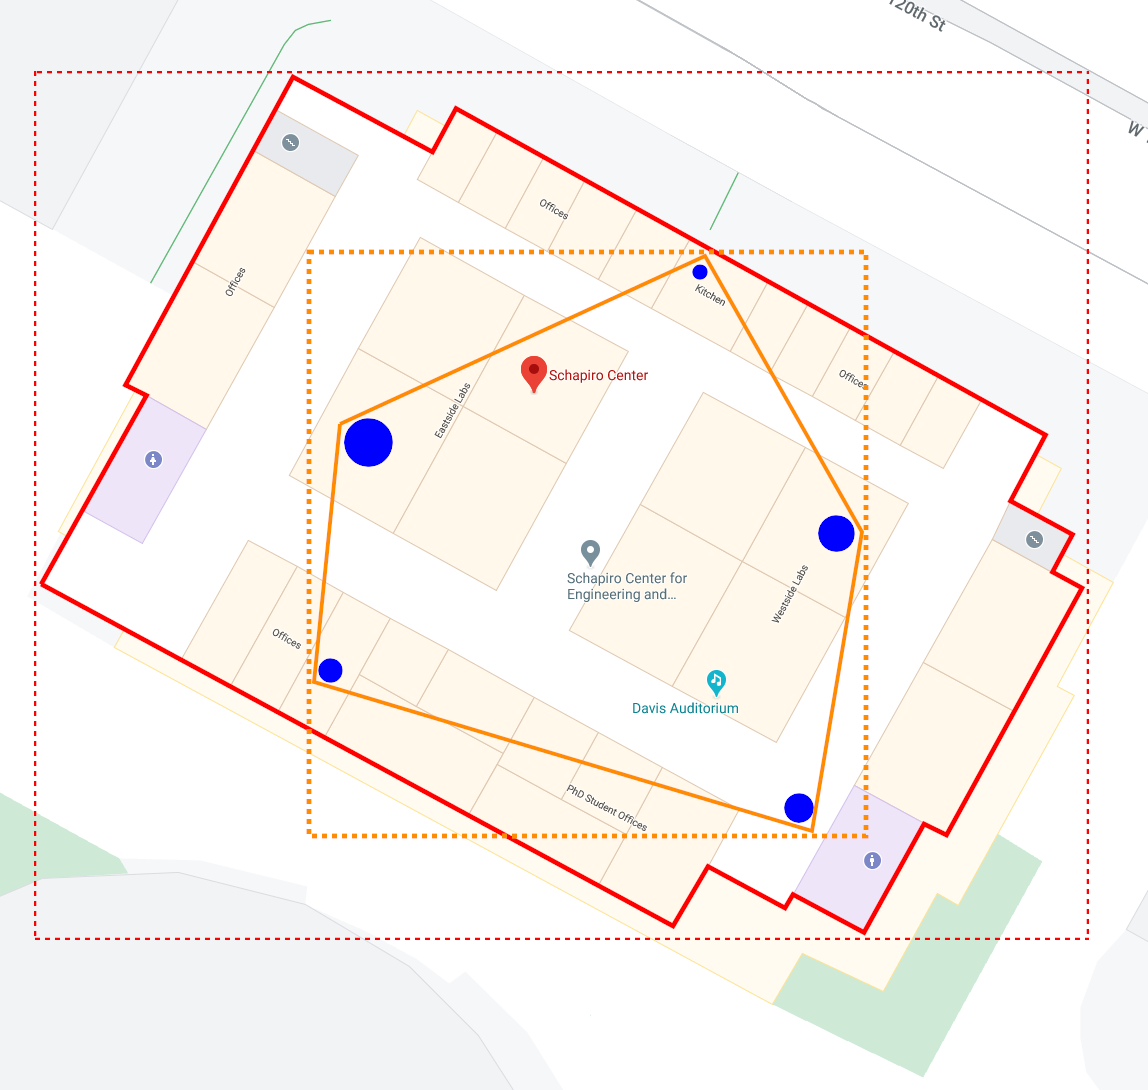
\includegraphics[width=1\linewidth]{figs/acps-coverage.png}%
    \caption{Device location estimates (blue), computed coverage region (orange), manually configured coverage region (red). Corresponding bounding boxes are shown with dotted lines.}\label{fig:acps-coverage}%
\end{figure}


An \gls{acps} is a collection of networked sensors, actuators, and related infrastructure managed by a common administrative entity. \cref{fig:acps} shows the conceptual internal architecture of the \gls{acps}. The sensors in a smart home would typically belong one \gls{acps}. The infrastructure on a large university campus may be divided among several \glspl{acps}, e.g., by building or department. Event in small deployments it may be advantageous to operate multiple related \glspl{acps} to limit the scope of potential failures or to split the infrastructure into public and private.

Each device within the \gls{acps} is associated with a \emph{storage node}. The node provides persistent storage and a query interface for the data (measurements) generated by associated devices. The association is administrative and can change over time. While it might be best to place the storage node close to the sensors, e.g., in the same \gls{lan}, it is not required. The storage node could also be provided in the form of a cloud-based service communicating with its associated sensors over a \gls{wan}. The former approach can be realized by placing the storage on an \gls{iot} gateway. The latter accommodates sensors that maintain a persistent connection to manufacturer-operated cloud infrastructure.

The \gls{acps} includes various sensor protocol servers (\emph{MQTT Server} in \cref{fig:acps}), a local \gls{sql} database, and a \emph{storage agent} process. The agent obtains measurement data from sensors and writes the data into the database. The exact mechanism is out of scope and will depend on the facilities provided by sensor protocol (push or pull), the configuration of the \gls{acps}, and local administrator policies (e.g., measurement intervals).

% Some background on uncertainty/radius https://en.wikipedia.org/wiki/Geo_URI_scheme

We assume the \gls{acps} can estimate the \gls{wgs} 84\footnote{We choose \gls{wgs} 84 because that is the coordinate system used by the \gls{gps} and it is widely supported. Other coordinate systems exist. Alternatively, one could also use a planar (Euclidean) coordinate system which would simplify some of the math in \gls{sql} spatial.} coordinates of each associated device. It maintains a \emph{location estimate} for each device in the form of a $(latitude, longitude, uncertainty)$ triplet represented with a geo \gls{uri}~\cite{rfc5870}. The uncertainty component is expressed at a confidence of 95\% or higher. Geometrically, the location estimate can be represented by a disk with the radius $uncertainty$. A location estimate with large uncertainty (coarse location) as provided by, e.g., Wi-Fi or \gls{ip} address positioning services, is sufficient for many applications. The means through which location estimates are obtained is out of the scope of this paper. In \cref{fig:acps-coverage}, the location estimates are shown in blue.

% TODO: how is the published service descriptor authenticated?

The \emph{coverage region} of an \gls{acps} is a geographic region that fully contains the location estimates of all the devices associated with the \gls{acps}. The coverage region is not necessarily the smallest such region and could be defined administratively, e.g., based on a building floor plan. If not provided, the \gls{acps} computes its coverage region as a convex envelope over the location estimates of all of its devices. The coverage region may change over time as device come, go, or move. The coverage regions of multiple \glspl{acps} may overlap.

The \emph{bounding box} of an \gls{acps} is the minimum rectangle that fully contains the \glsfirst{acps}['s] coverage region. Both the coverage region and the bounding box are represented with a single GeoJSON~\cite{rfc7946} object. The "bbox" property must be present and represents the \gls{acps}['s] bounding box.

The \emph{service descriptor} of an \gls{acps} is a digitally signed \gls{json}~\cite{rfc8259} object that binds the \gls{acps}['s] coverage region with additional information describing the \gls{acps} such as its contact \gls{uri}, available sensor or actuator types, or a human-friendly name:
\begin{minted}[fontsize=\footnotesize]{JSON}
{ "@type": "ServiceDescriptor",
  "@context": "https://schema.org/SynSQL",
  "displayName": "IRT Lab Sensors",
  "lastUpdated": "<ISO timestamp>",
  "expires": "<ISO timestamp>",
  "coverageRegion": {
      "type": "Polygon",
      "bbox": [-10.0, -10.0, 10.0, 10.0],
      "coordinates": [] },
  "private": false,
  "contact": "wss://as-123.example.com:8443",
  "sensorTypes": [
      "urn:sensor:environmental:indoor",
      "urn:sensor:security",
      "urn:sensor:occupancy" ],
  "signature": {} }
\end{minted}

The \gls{acps} publishes (\emph{GeoPublisher} in \cref{fig:acps}) its service descriptor in the \gls{gd} discussed later.  The service descriptor should provide sufficient information for the clients to submit \gls{sql} queries to the \gls{acps}. We expect the service descriptors to be updated infrequently. The record provides attributes that enable caching.

The \gls{acps} provides a public \gls{sql}[-based] interface (\emph{SQL Processor} in \cref{fig:acps}) to the stored sensor and actuator data. An advantage of \gls{sql}[-based] interface, as opposed to just publishing the underlaying data, is that: 1) query computation can be moved to data, 2) dynamic access control policies can be applied, 3) information hiding can be enforced by the \gls{acps}. For simplicity, we assume that all \glspl{acps} use a common data model (discussed elsewhere in the paper).

At a minimum, the \gls{acps} must support basic standards-based \gls{sql}. The \gls{acps} can also indicate support for the spatial \gls{sql} extension in the published service descriptor. In that case, the \gls{acps} may receive \gls{sql} queries with spatial predicates\footnote{The idea here is that the \gls{acps} can indicate whether its storage node is willing to process spatial \gls{sql} queries. If it is, it may receive full \gls{sql} queries from query coordinators and will be expected to evaluate spatial predicates using supplied geospatial data. That allows moving the computationally expensive spatial operations from the coordinator to storage nodes, i.e., close to the data.}. This is useful, for example, if the \gls{acps}['s] storage node has private spatial objects, e.g., derived from a building floor plan. This feature allows the clients to query sensor measurements with respect to such data, without necessarily being able to obtain the spatial objects for privacy reasons.


\section{Geographic Discovery Service}\label{sec:geographic-discovery-service}

% Key features:
% =============
% decentralized with authority distributed across jurisdictions
% easy to deploy and operate with existing mechanisms (DNS, S3, Lambda)
% Computationally expensive operations performed only by seekers (billed to seeker's account)
% Easy for ASes to publish and maintain service descriptors (/tmp directory model)
% Incentivize sensor publishing by providing better access to sensors from remote ASes
% Efficient operation for large regions of interest (e.g., Manhattan)
% Provide transport services for ASes behind NAT
% Permission-less publishing mechanism (similar to the web)
% There needs to be support for both generic and cc registrars. By using cc registrars all
%   parts of the infrastructure can be made under one jurisdiction

% This is not a new problem. Various forms of geographic routing, addressing, and discovery have been explored by the vehicular area networking (VANET) community and others. There is the DNS LOC~\cite{} resource record type. The authors in \cite{} extended a DNS implementation to allow retrieving DNS RRs by longitude and latitude. Geocast~\cite{} is an geographic IPv6 addressing scheme for VANETs. SRI proposed to create the ".geo" TLD \cite{} for a hierarchy of "GeoRegistries", "Cell Servers", and "GeoRegistrars".

A key challenge for the architecture discussed in this paper is allowing \gls{sql} query coordinators to efficiently discover all \glspl{acps} related to a geographic region. Various forms of geographic routing, addressing, and discovery have been explored by the networking community~\cite{rfc1876,fioreze2011extending,meijerink2016efficient,dotgeo}. In this section, we describe the \gls{gd} designed for our application. The architecture and operational model of the \gls{gd} is partially inspired by the \gls{lost} protocol framework~\cite{rfc5582,rfc5222}.

\textbf{Design Considerations.} The \gls{gd} supports the delegation of authority over portions of the data. Specifically, it allows delegating responsibility over the data to existing trustees for country-code top-level domains. This provides support for a multi-stakeholder model of registration policy making. The service is easy to deploy and operate using existing network services (\gls{dns}, Amazon S3, cloud functions). Computationally expensive operations such as complex geographic object matching need to be performed only by seekers. The \gls{gd} is efficient for large (country-level) interest regions. An easy to use permission-less interface for publishers is provided.

\cref{fig:gd-arch} depicts the key building blocks. The \gls{gd} is a network service that allows \textit{GeoSeekers} (\gls{sql} query coordinators) via a \textit{GeoResolver} to discover \textit{GeoPublishers} (\glspl{acps}) by their coverage regions published into a shared database. Specifically, a seeker can discover all publishers with coverage regions that intersect\footnote{The term intersect here refers to the standard \gls{de9im} model.} the seeker's \textit{interest region}. The discovery operation is a two-step process. First, the resolver obtains a set of \textit{geoservers} that are authoritative for the region of interest. Second, the resolver interrogates the authoritative geoservers for relevant service descriptors. Both steps are discussed in detail in the following sections.

\begin{figure*}
  \centering
  \subfloat[Key components of the service.]{%
    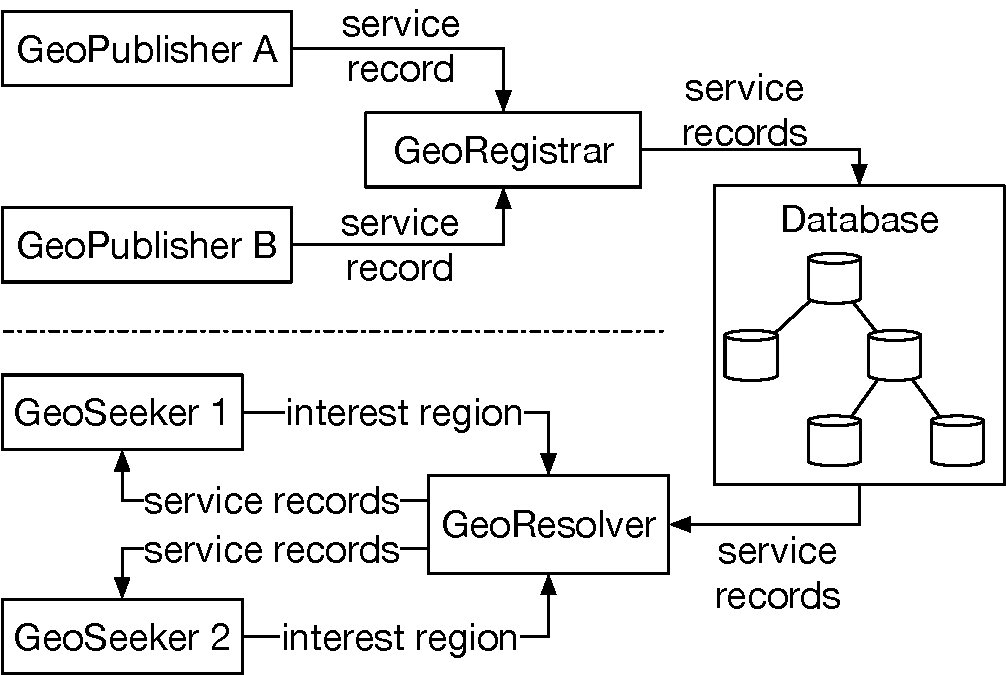
\includegraphics[width=0.45\linewidth]{figs/gd-arch.pdf}%
    \label{fig:gd-arch}%
  }
  \hspace*{\fill}
  \subfloat[Tree search.]{%
    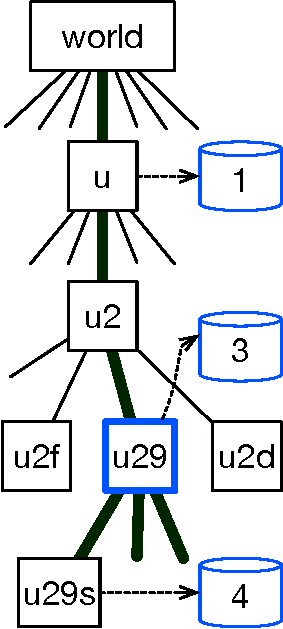
\includegraphics[width=0.13\linewidth]{figs/tree-search.pdf}%
    \label{fig:tree-search}
  }
  \hspace*{\fill}
  \subfloat[Geoserver delegation.]{%
    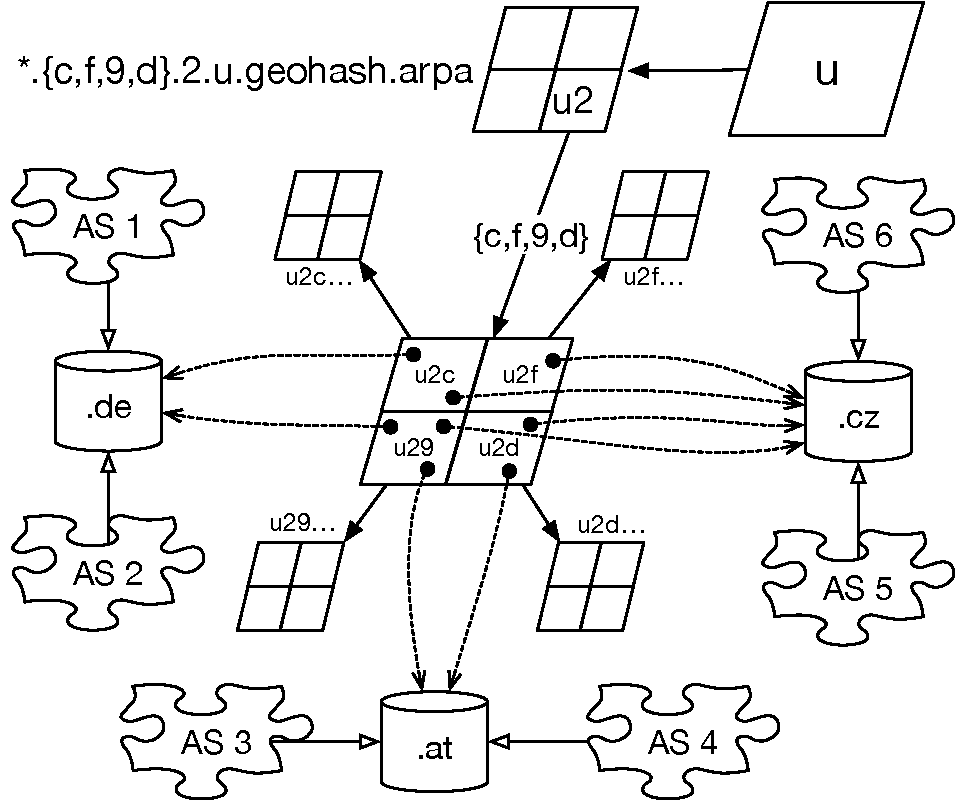
\includegraphics[width=0.36\linewidth]{figs/ddds.pdf}%
    \label{fig:coverage-region}
  }
  \caption{The architecture of the \glsfirst{gd}.}\label{fig:system-architecture}
\end{figure*}


\subsection{Discovering Geoservers}\label{sec:discovering-geoservers}

The world is divided into a hierarchy of cells according to the Geohash~\cite{geohash}algorithm. Each cell is identified by its Geohash identifier string. We organize the cells into a 32-ary tree. The tree root represents the entire world. The nodes immediately below the root correspond to the Geohash cells with identifier length 1. The nodes at the next lower level represent Geohash cells with identifier length 2, and so on. If the depth of the tree is 6, the leaves have 5 character long Geohash identifiers and the size of the corresponding geographic region is approximately \SI{5}{\kilo\metre}~x~\SI{5}{\kilo\metre}.

Each geoserver chooses a set of Geohash cells over which it will be authoritative. We envision per-country hierarchy of authoritative geoservers, similar to the country-code \gls{dns} zones. Such geoservers will choose the geohash cells that entirely cover the country\footnote{The exact (greedy) algorithm is described elsewhere in the paper}. The authoritative geoserver is then associated the corresponding nodes within the three. A server registered at tree node $X$ will become authoritative for the entire subtree rooted at $X$. More than one server may be authoritative for a subtree. In that case, the servers are distinguished by their country codes. \cref{fig:tree-search} and \cref{fig:coverage-region} illustrate the idea.

To find all the servers authoritative for a Geohash cell, the tree is traversed from the root to the node that represents the cell. The client notes any servers encountered in the nodes along the way. Once the target node has been reached, the client performs a search across the entire subtree rooted at the node, adding any discovered servers to the set. The resulting set may contain two types of authoritative servers: 1) servers whose coverage area includes the cell of interest, 2) servers whose coverage area lies within the cell of interest. In \cref{fig:tree-search} the cell of interest and the resulting authoritative servers are highlighted in blue. The search path is highlighted in bold.

\subsubsection{Database Implementation}\label{sec:database-implementation}

We propose to create a new \gls{dns} zone called \texttt{geohash.arpa}. The zone, to be administered in cooperation with the internet technical community. will be used to manage the association between geographic regions and the geoservers authoritative for the regions. The administrative procedures for the new zone can be similar to the procedures for managing \glspl{cctld} in the \gls{dns} root zone. The zone serves as the database for a new \gls{ddds}~\cite{rfc3401} application. Its records represent Geohash cells. For example, the Geohash cell ``dr72hvp'' is represented by the domain name \texttt{p.v.h.2.7.r.d.geohash.arpa}.

To make a geoserver authoritative for a chosen Geohash cell, two \gls{dns} \gls{naptr}~\cite{rfc3403} records must be created for it: one for the corresponding domain name, and one for the wildcard variant of the domain name. We expect such records to be created and modified very infrequently, e.g., as a result of geographic or political boundary changes. Thus, the \texttt{geohash.arpa} zone is suitable for extensive caching.

\begin{minted}[fontsize=\scriptsize]{text}
...
9.2.u   IN NAPTR 86400 10 10 "S" "GEO" geosrv-cz.example.com.
9.2.u   IN NAPTR 86400 10 10 "S" "GEO" geosrv-de.example.com.
9.2.u   IN NAPTR 86400 10 10 "S" "GEO" geosrv-at.example.com.

*.9.2.u IN NAPTR 86400 10 10 "S" "GEO" geosrv-cz.example.com.
*.9.2.u IN NAPTR 86400 10 10 "S" "GEO" geosrv-de.example.com.
*.9.2.u IN NAPTR 86400 10 10 "S" "GEO" geosrv-at.example.com.
...
\end{minted}

\subsubsection{Search Algorithm}\label{sec:search-algorithm}

The client constructs a domain name from the Geohash cell identifier, e.g., ``u29s'' becomes \texttt{s.9.2.u.geohash.arpa}, and searches the \gls{dns} for the corresponding \gls{naptr} records.

\subsection{Discovering Service Descriptors}\label{sec:discovering-service-records}

TBD.

\subsection{Publishing Service Descriptors}\label{sec:publishing-service-records}

The \gls{gd} is designed to make it easy for \glspl{acps} to publish their service descriptors. The process involves uploading a digitally signed \gls{json} document to the web and invoking an indexing service to insert the document into the AS database based on the record's bounding box. The web server could be an Amazon S3 bucket, a Github repository, or a service provided by a \gls{dns} registrar. The operational model is similar to the "/tmp" directory\footnote{Any user can create a file in /tmp. Only the user who created the file can remove the file.} in UNIX-like operating systems. Any \gls{acps} can submit a service descriptor to the \gls{acps} database\footnote{TODO: This approach may be vulnerable to data poisoning. Discuss and address this elsewhere in the paper.}. The corresponding secret key is required to update or delete the service descriptor.

%\subsection{Operational Example}\label{sec:operational-example}

%Consider a seeker trying to discover all \glspl{acps} within the Morningside Heights neighborhood. The seeker submits a geographic object representing the neighborhood's surface to a resolver. The resolver decomposes the object into a set of GeoHash~\cite{geohash} strings.

%Consider the situation in \cref{fig:bounding-boxes}. A search for \glspl{acps} that intersect Morningside Heights (orange) would yield \glspl{acps} 1 (red) and 2 (purple).

%Internally, the \gls{gd} service consists of two subsystems: 1) a \gls{dns}[-based] indexing database, 2) a set of authoritative servers. The indexing database allows the resolver to efficiently find authoritative servers. The authoritative server allows the seeker to discover publishers in its coverage region. The \gls{dns} service allows delegation across jurisdictions. The authoritative server is similar to a TLD \gls{dns} registry. External registrars may provide services that allow publishers to publish service descriptors. This architecture is actually designed to make it possible for existing \gls{dns} registries and registrars to participate in the service without having to deploy new functionality.

%Internally, the \gls{gd} service operates on bounding boxes. The resolver computes a bounding box for the geographic object supplied by the seeker and searches the database for \glspl{acps} with intersecting bounding boxes. This simplification makes the \gls{gd} service scalable but yields false positives (\cref{fig:bounding-boxes}) that are filtered out by the resolver.

% Publishing a service descriptor involves uploading the \gls{json} document somewhere where it can be found and invoking an indexing service that will properly index it into the \gls{acps} database based on the record's bounding box.

%\subsubsection{ACPS Server Delegation}\label{sec:as-server-delegation}

%We use the \gls{ddds}~\cite{rfc3401} to map geographic regions to \gls{acps} servers responsible for the region. Note that a region can be resolved to multiple authoritative \gls{acps} servers, e.g., a region at the border of two countries. The application can query both or it can configured with a country identifier that determines which one to pick.

%The application unique string is the geohash of the regions bounding box. A single bounding box may overlap with up to four geohash regions. In that case, the application will end up with multiple application unique strings and needs to resolve each of them separately.

%The \gls{gd} service consists of hierarchically organized independently operated servers. At the top of the hierarchy is a small set of well-known root servers. The root servers are similar to \gls{dns} root servers and must be synchronized with each other. All clients (resolvers) must known the root servers. The root servers partition the world into large geographic regions and assign an authoritative \gls{gd} server to each region. The server's authoritative region is called a \textit{service region}. Each server then delegates portions of its service region to other \gls{gd} servers, and so on. We envision a fairly flat hierarchy of servers, similar to \gls{dns}. Unlike in \gls{dns} where delegation is based on domain labels, the delegation in \gls{gd} is based on spatial relationships of service regions.

%\gls{gd} clients (query resolvers in our architecture) communicate with the \gls{gd} service via a resolver. The resolver is pre-configured with a domain name and uses the usual \gls{dns} mechanisms (\gls{naptr}, \gls{srv}) to locate the \gls{gd} for its domain. The resolver discovers \gls{gd} servers, performs service descriptor caching, and maintains persistent light-weight communication sessions with selected \glspl{as}.

%The client requests service from the \gls{gd} by submitting a \textit{Lookup} request to its resolver. The request contains a geospatial region of interest (GeoJSON) and (optionally) desired sensor types:
% \begin{minted}[fontsize=\footnotesize]{JSON}
% { "@type": "ASLookup",
%   "@context": "https://schema.org/SynSQL",
%   "interestRegion": {
%       "type": "Polygon",
%       "bbox": [-10.0, -10.0, 10.0, 10.0],
%           "coordinates": [] },
%   "sensorTypes": [
%       "urn:sensor:environmental" ] }
% \end{minted}
%The \gls{gd} can reject the request if the submit region of interest is too complex or if it is missing the "bbox" property. In the \gls{gd} architecture, complex geographic object matching is always left to the resolver for scalability reasons.

%The \gls{gd} consults its database of service descriptors published by \glspl{acps}. It returns to the client the service descriptors of all \glspl{acps} that intersect (i.e., are not disjoint) the region of interest in the standard \gls{de9im}~\cite{simple-feature-access}. In other words, an \gls{acps} will be included in the result set if and only if its coverage region has coordinates in common with the bounding box of the client's region of interest. Restricting the matching algorithm to bounding boxes greatly simplifies the operation of the \gls{gd}, at the expense of producing false positives, i.e., \glspl{acps} that do not intersect the region of interest included in the result set. The returned service provide all the information necessary for the client to submit \gls{sql} queries to the corresponding \glspl{acps}.

%The client is expected to cache and reuse the result set for the same region interest.

% How to scale the ASD?
% How to deal with public and private ASes?

\section{Query Coordinator}\label{sec:query-coordinator}

% Discovery of ASD servers?
% Caching of returned data (indicate the region for which the same answer would be returned)
% Recursive and iterative query resolution

\subsection{Query Processing}\label{sec:query-processing}

Consider an application to monitor \href{https://www.epa.gov/pm-pollution}{\gls{pm2.5} pollution} trends in a region, e.g., \href{https://www.openstreetmap.org/relation/8398079}{Morningside Heights} neighborhood in New York City. Suppose many \gls{pm2.5} sensors have been installed in the neighborhood by individual residents, organizations, or city administration, and that measurement data from those sensors are available to the public. In this section, we discuss how the application could obtain measurement data in a distributed manner using a standard \gls{sql}~\cite{sql} query such as:
\begin{minted}[fontsize=\footnotesize]{SQL}
  SELECT MAX(measurements.data::numeric)
  FROM measurements as M, spatial as S
  WHERE
    S.name = 'Morningside Heights'
    AND ST_Contains(S.bounds, M.loc)
    AND M.quantity = 'PM2.5'
\end{minted}

Refer to \cref{fig:system-architecture} for a conceptual diagram of the query processing architecture. To obtain the required measurement data, the application issues a \gls{sql} \textit{SELECT} query to a pre-configured \gls{sql} proxy. The proxy can be provided by the application's execution environment, e.g., the cloud infrastructure the application is running on.

If the \gls{sql} query does not refer to a virtual \textit{measurements} table or if it does not contain spatial predicates~\cite{sql-spatial,simple-feature-access}, the proxy forwards the query to a pre-configured local \gls{sql} database. The database is also provided by the application's execution environment. It contains geographic objects, application-specific data, and may also serve as a cache for previously obtained measurement data.

If the \gls{sql} query refers to the virtual \textit{measurements} table and contains spatial predicates, the proxy executes the query in a distributed manner. First, it retrieves the representations of relevant spatial objects from the local \gls{sql} database. Second, the proxy submits the representations to the \gls{gd}. The \gls{gd} returns a set of \glspl{acps} likely to have relevant measurement data. Third, the proxy transforms the original \gls{sql} query into sub-queries and forwards those to the \glspl{acps}. Finally, the proxy merges and aggregates partial results from the \glspl{acps} for the application.

Our architecture is designed to support queries over large geographic regions and the polygon representations involved in such queries could be quite complex\footnote{Measured by the number of vertices in the objects's boundary polygon.}. For example, the boundary polygon for Morningside Heights neighborhood obtained from OpenStreetMaps has 89 points. The boundary polygon for Manhattan borough, the immediate enclosing spatial object, contains almost 1,700 points.

To alleviate the need for the \gls{gd} to process complex spatial objects, the \gls{sql} proxy runs a polygon simplification algorithm, similar to~\cite{song2011polygon}, on the spatial objects submitted to the \gls{gd}. The algorithm must be carefully designed to fully contain the original polygon entirely\footnote{Violating this requirement may result in an incomplete \gls{acps} set, missing sensor measurement data, and incorrect results.}. This optimization may result in false positives, i.e., measurement data that should have been excluded from the result set. Thus, the \gls{sql} proxy must filter the data returned from \glspl{acps} using the original (not simplified) polygons. This important optimization shifts the burden of complex spatial object processing from the \gls{gd} to the \gls{sql} proxy and thus the application executing the \gls{sql} query.

\section{Data Model}\label{sec:data-model}

\subsection{Temporal Semantics}\label{sec:temporal-semantics}

% https://www.postgresql.org/message-id/CA+renyUb+XHzsrPHHR6ELqguxaUPGhOPyVc7NW+kRsRpBZuUFQ@mail.gmail.com
% standard SQL system-versioned tables
% select * from foo as of system time now()-10s

\subsection{Spatial Objects}\label{sec:spatial-objects}

\textit{Discuss how spatial objects are stored in the local \gls{sql} database, what they represent, where they come from, and what kind of processing  must be performed on data obtained, e.g., from OpenStreetMaps}.

\subsection{Sensor Measurement Data}\label{sec:sensor-measurements}

\textit{Discuss the design of the virtual measurements table, including how various types of measurements (discreet and continuous) are stored in the virtual table.}

\section{Event Notification}\label{sec:event-notification}

\begin{figure*}
  \centering
  \subfloat[Polygon for Manhattan borough.]{%
    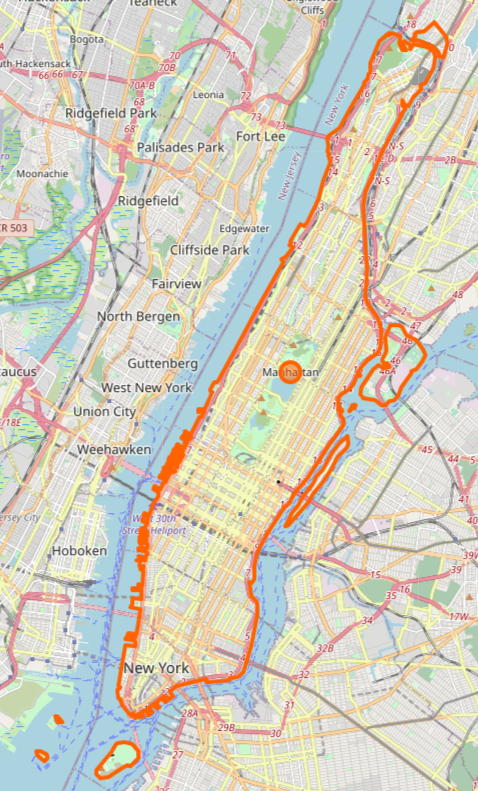
\includegraphics[width=0.29\linewidth,valign=c]{figs/manhattan-ploygon.png}%
    \label{fig:manhattan-polygon}%
  }
  \hspace*{\fill}
  \subfloat[Polygon for Morningside Height Neighborhood.]{%
    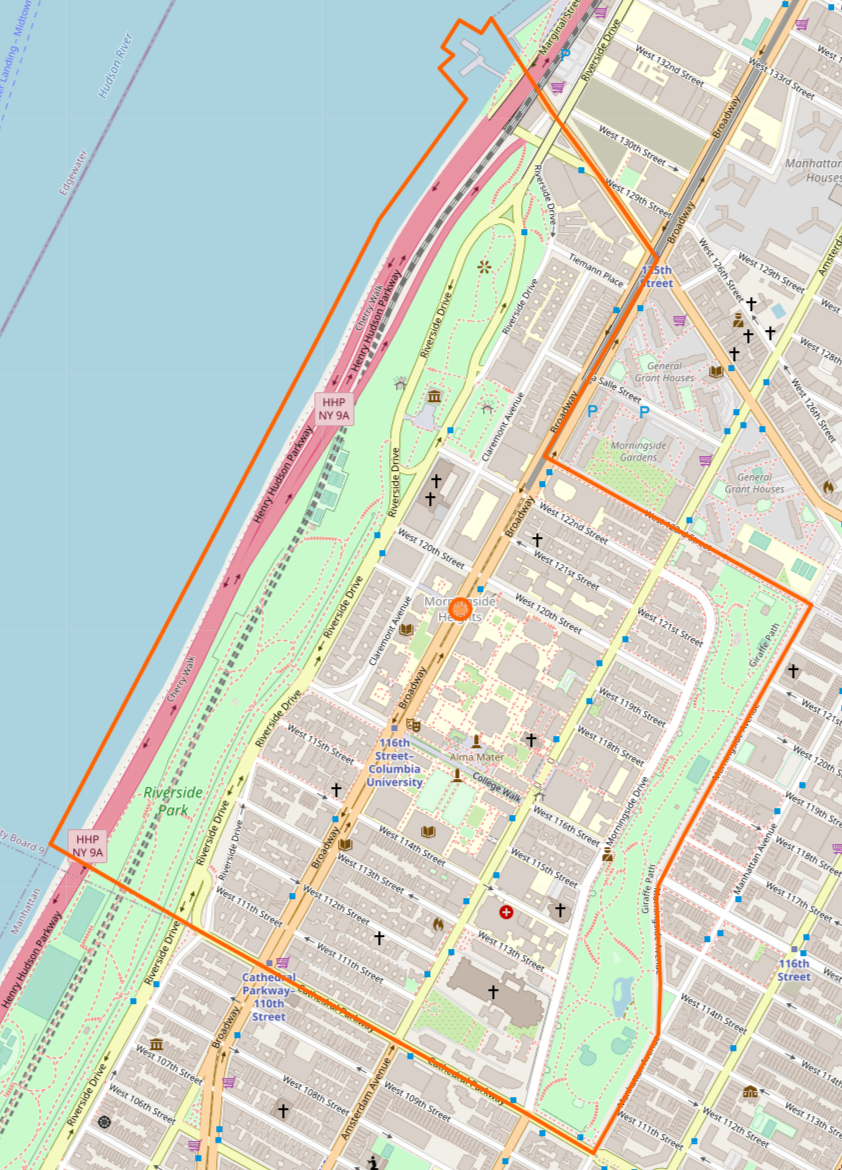
\includegraphics[width=0.3\linewidth,valign=c]{figs/morningside-heights-polygon.png}%
    \label{fig:morningside-heights-polygon}%
  }
  \hspace*{\fill}
  \subfloat[3D model of Shapiro Center for Engineering on Columbia University campus.]{%
    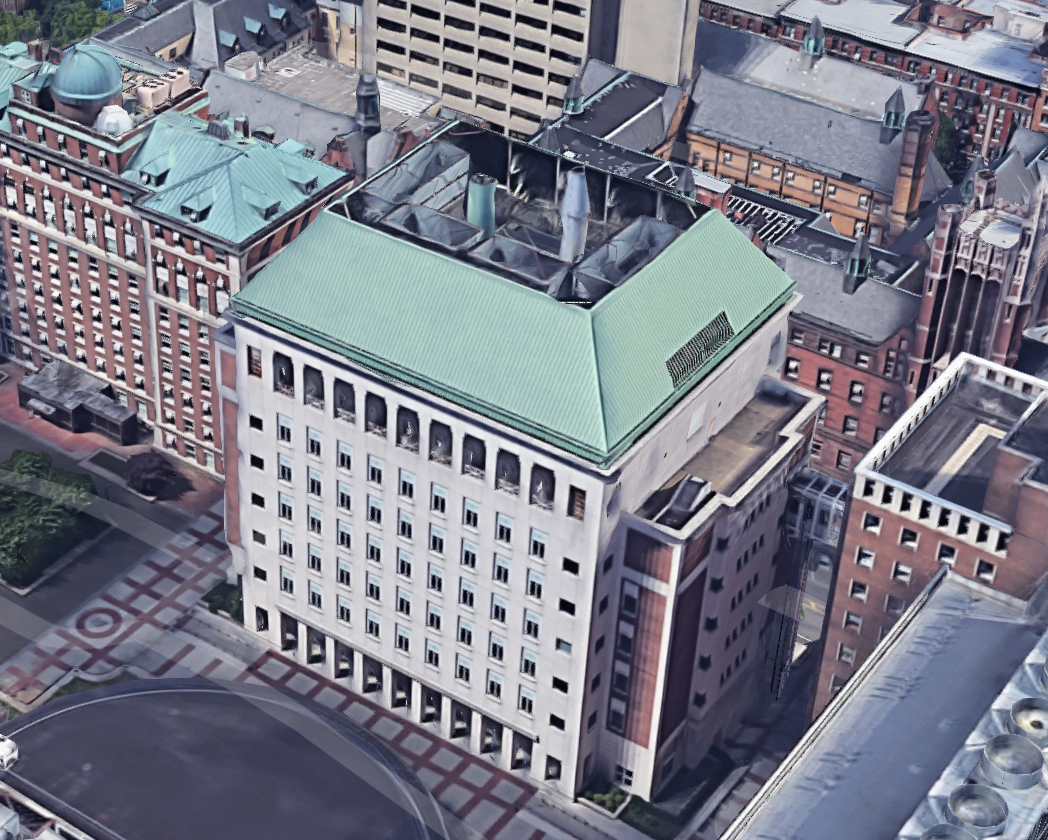
\includegraphics[width=0.4\linewidth,valign=c]{figs/cepsr-3d.png}%
    \label{fig:cepsr-3d}%
  }
  % \subfloat[]{%
  %   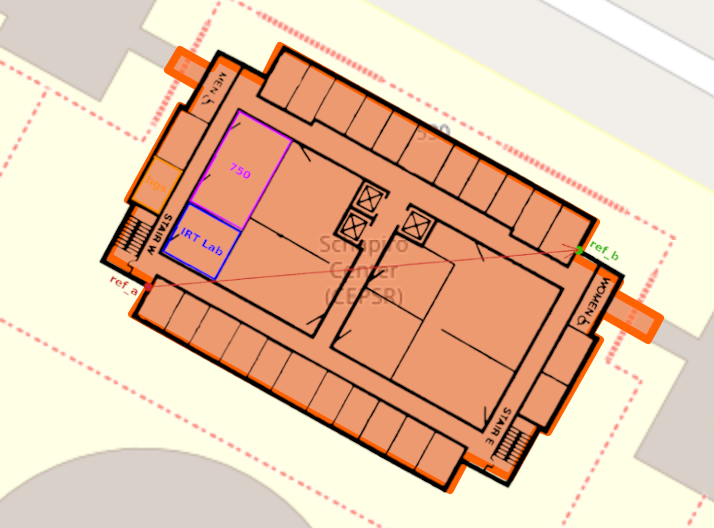
\includegraphics[width=0.36\linewidth]{figs/cepsr_floorplan_superimposed.png}%
  %   \label{fig:cepsr-floorplan}%
  % }
\end{figure*}

\section{Conclusion}\label{sec:conclusion}

\subsection{Future Work}\label{sec:future-work}

Similar basic mechanism could work for updating some kinds of actuators (via \gls{sql} \textit{UPDATE}). Particularly, the reliability of the updates could be justified in the face of conflicts or failing actuator updates. The ACID semantics might be useful, or a model similar to \href{https://dl.acm.org/doi/pdf/10.1145/2491245}{Google Spanner}.

\bibliographystyle{IEEEtran}
\bibliography{bibs/references,bibs/rfc,bibs/db}

% \begingroup
% \parindent 0pt
% \parskip 1ex
% \def\enotesize{\footnotesize}
% \theendnotes
% \endgroup

\end{document}